

The program accepts an event log and an optional process model, e.g. a Petri net, as inputs and returns a corresponding translucent event log as output. Users have the option to select from various methods of log generation, will be specified below. Mainly, these methods can be classified in two categories: top-down approaches which require a Petri net, and bottom-up approaches which solely need the event log.

In order to provide a user-friendly interface, we implement a web application. The following sections describe the software specification, architecture, and its features. The comprehensive source code is publically available on GitHub\footnote{https://github.com/biscimus/Translucify}\footnote{https://github.com/biscimus/Translucify-Transformer-Service}.

\section{Software Architecture}

In the following sections, we briefly describe the technical architecture used for \emph{Translucify}. The architecture can be partitioned into two main components, the backend and the frontend. The backend houses the actual algorithms used to extend the event log with enabled activities, while the frontend provides a UI for user interaction.

\subsection{Backend}

The backend was implemented with Python using the Flask\footnote{www.flask.palletsprojects.com/en/3.0.x/} framework. Flask is fitting for our use case as it is a lightweight framework providing a minimalistic set of features needed to build API calls.

Behind the API handlers, the backend logic is dependent on \texttt{PM4Py} \cite{pm4py}, a novel, rapidly established process mining library written for the Python programming language. Other than \texttt{PM4Py}, standard libraries necessary for machine learning and data processing, such as \texttt{NumPy} \cite{numpy}, \texttt{Pandas} \cite{pandas}, and \texttt{Scikit-learn} \cite{scikit-learn} were used. The choice of using Python for building the backend was an intentional decision in order to incorporate these libraries natively into the backend.

For the database, SQLAlechemy\footnote{www.sqlalchemy.org} was used as an object relational mapping (ORM) tool to model the database. It was chosen due to its seamless compatibility with Flask using the Flask-SQLAlchemy extension and its ease of usage.

The database stores event log entities and their corresponding translucent event log entities. Since the event logs tend to be large, the actual event logs are stored in the file system, while the database only keeps track of the metadata, such as the file path, name, and type of the event logs. Translucent event log entities have an extra attribute \texttt{is\_ready} in order to indicate whether the computation is complete. The database schema is depicted in Figure \ref{fig:db_schema}.

\tikzset{multi attribute/.style={attribute, double distance=1.5pt}}
\tikzset{derived attribute/.style={attribute, dashed}}
\tikzset{total/.style={double distance=1.5pt}}
\tikzset{every entity/.style={draw=orange, fill=orange!20}}
\tikzset{every attribute/.style={draw=MediumPurple1, fill=MediumPurple1!20}}
\tikzset{every relationship/.style={draw=Chartreuse2, fill=Chartreuse2!20}}
\newcommand{\key}[1]{\underline{#1}}

\begin{figure}[H]
    \centering
    \begin{tikzpicture}[node distance=5em]
        \node[entity](eventlog){\texttt{EventLog}};
        \node[attribute](pid)[left of=eventlog, xshift=-0.5cm]{\texttt{\key{id}}} edge(eventlog);
        \node[attribute](name)[above left of=eventlog]{\texttt{name}} edge(eventlog);
        \node[attribute](type)[above right of=eventlog]{\texttt{type}} edge(eventlog);
        \node[attribute](filepath)[right of=eventlog, xshift=1cm]{\texttt{file\_path}} edge(eventlog);
        \node[relationship](has)[below of=eventlog]{\texttt{has}} edge(eventlog);
        \node[entity](translucenteventlog)[below of=has]{\texttt{TranslucentEventLog}} edge[total](has);
        \node[attribute](tid)[left of=translucenteventlog, xshift=-1.5cm]{\texttt{\key{id}}} edge(translucenteventlog);
        \node[attribute](tname)[below left of=translucenteventlog, xshift=-1cm]{\texttt{name}} edge(translucenteventlog);
        \node[attribute](tisready)[below of=translucenteventlog]{\texttt{is\_ready}} edge(translucenteventlog);
        \node[attribute](ttype)[below right of=translucenteventlog, xshift=1cm]{\texttt{type}} edge(translucenteventlog);
        \node[attribute](tfilepath)[right of=translucenteventlog, xshift=2cm]{\texttt{file\_path}} edge(translucenteventlog);
    \end{tikzpicture}
    \caption{Entity-relationship diagram of the database schema.}
    \label{fig:db_schema}
\end{figure}

\subsection{Frontend}

The frontend is a web application built with React \cite{react}. The application leverages Mantine \footnote{https://mantine.dev/} as its UI library, TanStack Router \footnote{https://tanstack.com/router/latest} for routing and TanStack Query \footnote{https://tanstack.com/query/latest} for asynchronous state management. The frontend application is responsible for sending \& receiving requests \& responses with the backend, parsing \& rendering the data, and finally to provide a user-friendly interface for the user to interact with the application.

The web application will start with an interface where the user can upload an event log, with a choice between CSV and XES. After uploading the event log, different methods of translucent log annotation will be available. The user can select the method and the corresponding necessary parameters. After the log generation is complete, the user can download the log either in a CSV or an XES format.

\section{Software Features}

The following section outlines some technical features employed to implement the software architecture. It also describes the sequence flows within application between the frontend and the backend.

\subsection{GPU Computing}
For the transformer variant, in order to train the transformer model, a GPU access was necessary due to the high computational requirements. In a local setting, the program would take an extraordinary amount of computing time, or in other cases simply terminate due to insufficient memory.

In order to solve this issue, a connection to the remote PADS HPC Cluster needed to be established. Inside the cluster, a Flask microservice was set up analogously to the local setup. Using SSH tunneling, all requests regarding the transformer model were then forwarded to the remote server. After the computations are finished, the results from the remote server were subsequently delivered back to the main application running in the local server. Figure \ref{fig:ssh_tunneling} illustrates the SSH port forwarding setup.

\begin{figure}
    \centering
    \begin{tikzpicture}

        % Computer icons
        \node[label=below:\texttt{localhost}] (local) {\fcComputer{0.1}{black}{0.5}};
        \node[right of=local, xshift=6cm, label=below:\texttt{Remote GPU Server}] (remote) {\fcComputer{0.1}{black}{0.5}};

        % Ports
        \node[below of=local, rectangle,  yshift=-1cm, fill=yellow] (localport3000) {\texttt{Port :3000}};
        \node[below of=remote, rectangle, yshift=-1cm, fill=yellow] (remoteport5000) {\texttt{Port :5000}};
        \node[below of=localport3000, rectangle, fill=yellow] (localport5000) {\texttt{Port :5000}};
        \node[below of=remoteport5000, rectangle, fill=yellow] (remoteport3000) {\texttt{Port :3000}};

        % Arrows
        \draw[thick, ->, >=stealth] (localport3000) -- (remoteport5000) node[midway, above, xshift=-0.25cm] {\texttt{request}};
        \draw[thick, ->, >=stealth] (remoteport3000) -- (localport5000) node[midway, above, xshift=-0.25cm] {\texttt{callback}};

        % Borders
        \draw[dotted, thick, rounded corners] ($(local.north west) + (-0.5, 0.5)$)  rectangle ($(localport5000.south east) + (0.5, -0.5)$);
        \draw[dotted, thick, rounded corners] ($(remote.north west) + (-1, 0.5)$)  rectangle ($(remoteport3000.south east) + (1, -0.5)$);

    \end{tikzpicture}
    \caption{SSH Port Forwarding.}
    \label{fig:ssh_tunneling}
\end{figure}

\begin{figure}
    % Include a picture
    \centering
    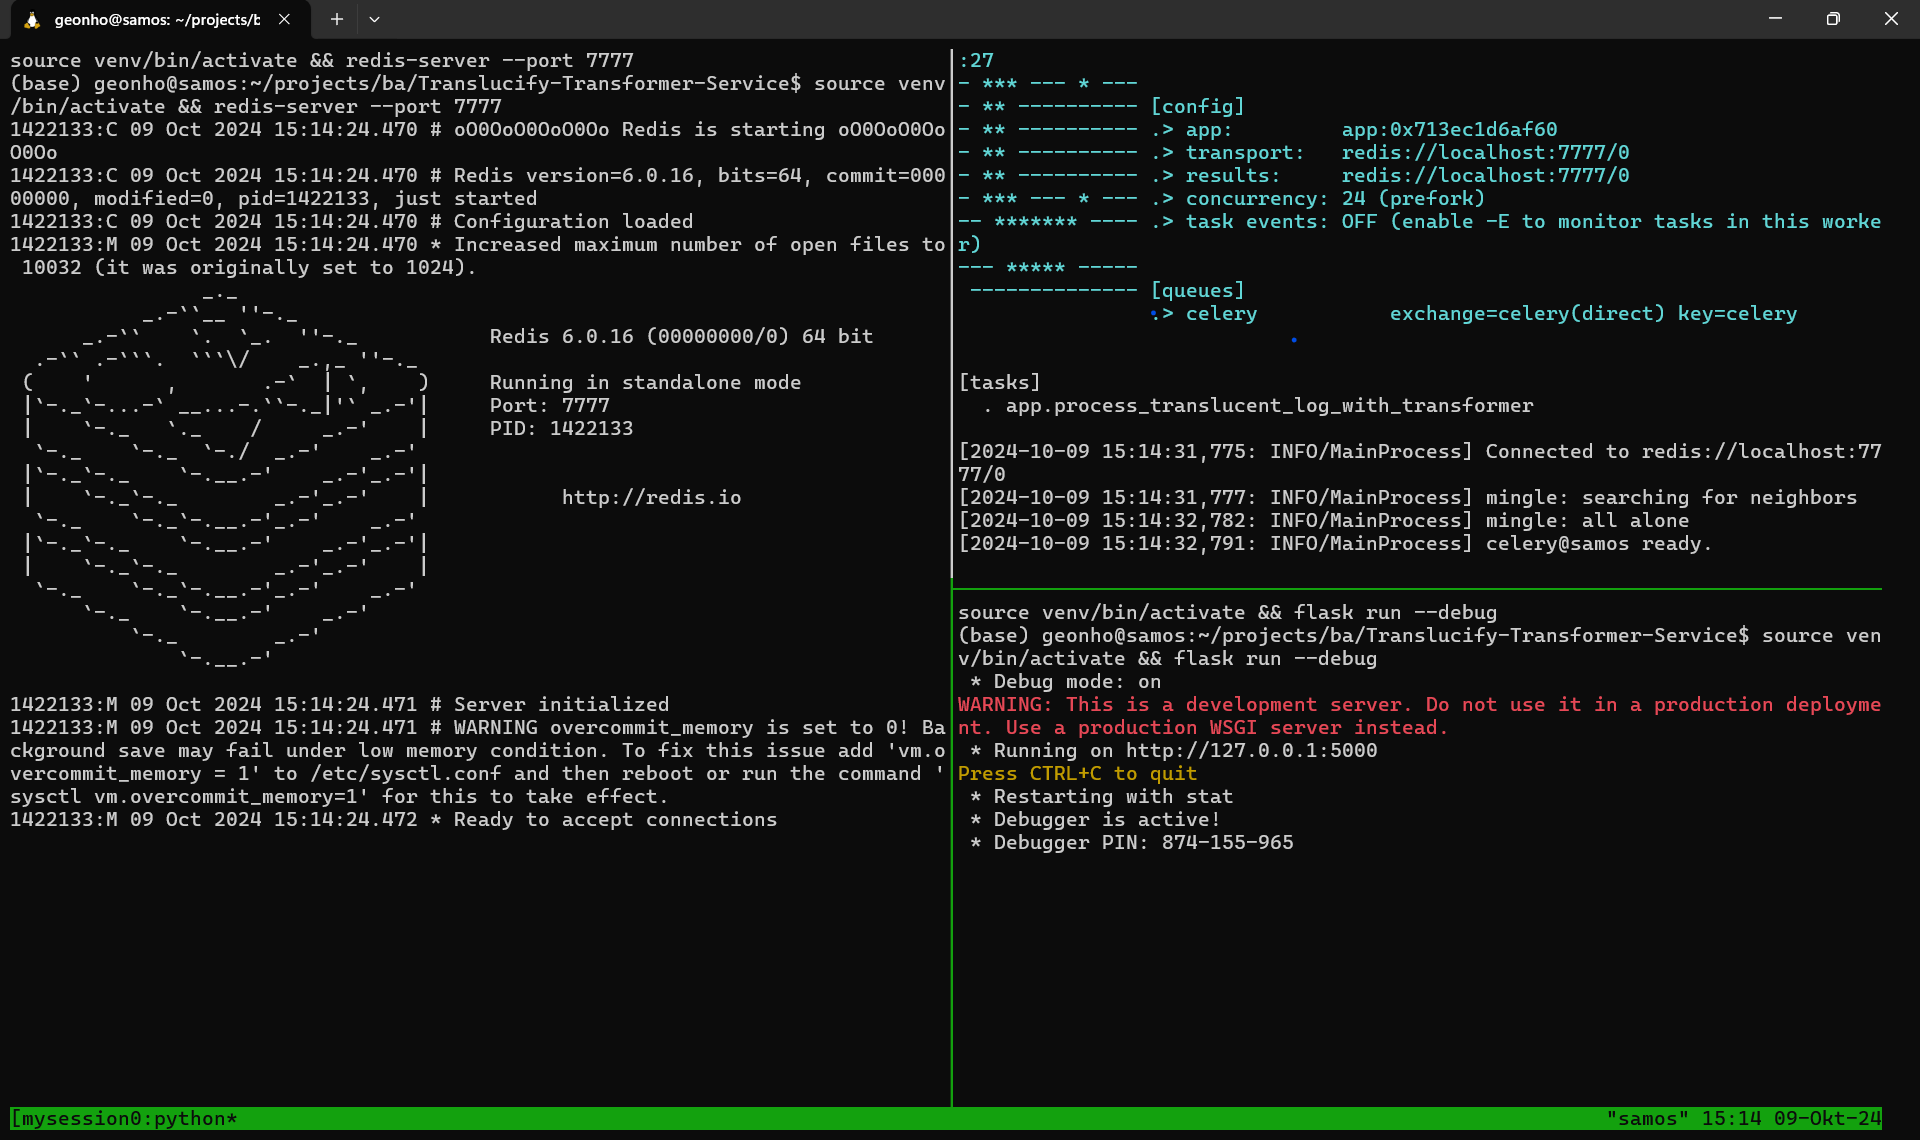
\includegraphics[width=\textwidth]{figures/remote-service.png}
    \caption{Screenshot of the remote service running on the HPC Cluster. In each of the three separate tmux terminals, the Redis server (left), the Celery worker (top right), and the Flask server (bottom right) are running.}
    \label{fig:remote_service}
\end{figure}

A screenshot of the remote service is available in Figure \ref{fig:remote_service}.

\subsection{Asynchronous Task Distribution}
All requests from the frontend are processed by request handlers of Flask. A particular issue we encountered is this case was the excessive computation time for each algorithm run in the backend. As a result, when attempting to run the algorithms directly on the request handlers in Flask, the server would block all other requests until the current computation was finished, making the application unresponsive and bluntly unusable. To mitigate this issue, we incorporated a distributed task queue using Redis\footnote{https://redis.io/} and Celery\footnote{https://pypi.org/project/celery/}.

Celery is a distributed system to split up computation in tasks and to assign these to subprocesses, known as workers. Redis is used as a \emph{message broker} so that the Celery client can delegate the tasks to the workers. Upon receiving a request, the Flask server will pass on the task to the Celery client, which will then push the task to a Redis Message Queue. The Celery workers will then pick up the task from the queue and execute it. Compared to the setup where all tasks are handled directly in the request handlers, this setup allows for a non-blocking behavior of the server, as the tasks are executed in the background by other processes, thereby preventing the application from freezing.

The overall application architecture is depicted in Figure \ref{fig:app_architecture}.

\begin{figure}
    \centering
    \begin{tikzpicture}[node distance=2cm]
        \foreach \i in {0,1} {
            \begin{scope}[xshift=\i*7.65cm]
                
                % Backend (API Server)
                \node[yshift=-1cm, label=below:\texttt{Server}] (backend\i) {\Huge \faServer};
                
                % Database
                \node[below of=backend\i, yshift=-1cm, label=below:\texttt{Database}] (database\i) {\Huge \faDatabase};
                
                % Message Queue
                \node[cylinder, draw, fill=red!50, text centered, minimum height=5em, shape aspect=0.75, right of=backend\i, label={[label distance=0.25cm]below:\texttt{Redis MQ}}] (queue\i) {\texttt{Tasks}};

                % Celery
                \node[right of=queue\i, xshift=0.55cm, label=below:\texttt{Celery}] (celery\i) {\Huge \faSitemap};

                % Worker 1
                \node[below of=celery\i, rectangle, yshift=0.5cm, fill=yellow] (worker1\i) {\texttt{Worker 1}};

                % Worker 2
                \node[below of=worker1\i, yshift=1cm, rectangle, fill=yellow] (worker2\i) {\texttt{Worker 2}};

                % dots
                \node[below of=worker2\i, yshift=1cm] (dots\i) {\Huge $\vdots$};

                % Worker n
                \node[below of=dots\i, yshift=1cm, rectangle, fill=yellow] (workern\i) {\texttt{Worker n}};

                % Arrows
                \draw[thick, <->, densely dotted, >=stealth] ($(backend\i) + (0, -1)$) -- (database\i);
                \draw[thick,->,>=stealth] (backend\i) -- (queue\i);
                \draw[thick,->,>=stealth] (queue\i) -- (celery\i);
                \draw[thick, <->,densely dotted, >=stealth] ($(worker1\i) + (-1.35, -1.5)$) -- (database\i);

                % Borders
                
                % Application border
                \draw[dotted, thick, rounded corners] ($(backend\i.north west) + (-0.5, 1)$)  rectangle ($(workern\i.south east) + (0.75, -1)$);

                % Celery border
                \draw[thin, rounded corners] ($(celery\i.north west) + (-0.65, 0.5)$) rectangle ($(workern\i.south east) + (0.35, -0.5)$);
            \end{scope}
        }

        % Frontend (browser)
        \node[above of=backend0, yshift=1.5cm, label=below:\texttt{Browser}] (frontend) {\Huge \faDesktop};

        % User
        \node[dave, above of=frontend, yshift=1cm, label=below:\texttt{User},minimum size=1cm] (user) {};

        \draw[thick,<->,>=stealth] ($(user) + (0, -1.5)$) -- (frontend);
        \draw[thick,<->,>=stealth] ($(frontend) + (0, -1.25)$) -- (backend0);

        % SSH connection
        \node[draw, cloud, cloud puffs=11, cloud puff arc=120, aspect=2, right of=frontend, xshift=4.5cm] (sshcloud) {\texttt{SSH Tunneling}};

        \draw[densely dotted, >=stealth, out=120, in=90] (sshcloud.west) to[out=220, in=90] ++(-2,-2); % Left arm
        \draw[densely dotted, >=stealth, out=90, in=90] (sshcloud.east) to[out=320, in=90] ++(2,-2);  % Right arm

        % Labels
        \node[below of=database0, xshift=2.5cm, yshift=-0.4cm] {\texttt{Local}};
        \node[below of=database1, xshift=2.5cm, yshift=-0.4cm] {\texttt{Remote}};
    \end{tikzpicture}
    \caption{Application Architecture}
    \label{fig:app_architecture}
\end{figure}

\subsection{Multivariable Regression With Petri Nets}

After the user selection, the client sends a request to the server to obtain the columns of the event log. After receiving the list of columns, the user subsequently selects a set of data columns to be used for the multivariable regression, while simultaneously indicating whether the columns are numerical or categorical. After the selection is complete, the client sends a request to the server to initiate the computation with corresponding columns. After the computation is terminated, the backend flips the \texttt{is\_ready} boolean attribute of the translucent event log entity.

The complete sequence is depicted in Figure \ref*{fig:sd_petri_net}.

\begin{figure}[H]
    \centering
    \begin{tikzpicture}[node distance=6cm,auto,>=stealth']
        \node[fill=yellow] (server) {\texttt{Server}};
        \node[left = of server, fill=yellow] (client) {\texttt{Client}};
        \node[below of=server, node distance=5cm] (server_ground) {};
        \node[below of=client, node distance=5cm] (client_ground) {};
        %
        \draw (client) -- (client_ground);
        \draw (server) -- (server_ground);
        \draw[->] ($(client)!0.25!(client_ground)$) -- node[above,scale=1,midway]{\texttt{\textbf{GET} /event-log/<id>/columns}} ($(server)!0.25!(server_ground)$);
        \draw[<-] ($(client)!0.35!(client_ground)$) -- node[below,scale=1,midway]{\texttt{\textcolor{blue}{columns}}} ($(server)!0.35!(server_ground)$);

        \draw[->, rounded corners=5pt] ($(client)!0.45!(client_ground)$) -- (-8, -2.25) -- (-8, -3.5) -- node[left,scale=1,midway, xshift=-0.25cm, yshift=0.75cm]{\texttt{Choose data columns}} ($(client)!0.70!(client_ground)$);

        \draw[->] ($(client)!0.80!(client_ground)$) -- node[above,scale=1,midway]{\texttt{\textbf{POST} /event-log/<id>/petri-net}} node[below, scale=1, midway]{\texttt{\textcolor{blue}{data column config}}} ($(server)!0.80!(server_ground)$);
    \end{tikzpicture}
    \caption{Client-server sequence diagram for the Petri net variant.}
    \label{fig:sd_petri_net}
\end{figure}

\subsection{Multivariable Regression with Prefix Automata}

The user sequence for multivariable regression with prefix automata is analogous to the Petri net variant for the most part. An additional step, however, is required in order to fine-tune the prefix automaton. After the data column selection step, the server computes a prefix automaton. The user then is able to fine-tune the prefix automaton by merging states. After the user is satisfied with his custom fine-tuned automaton, the client sends a request to the server to initiate the regression computation.

The complete sequence is depicted in Figure \ref*{fig:sd_prefix_automaton}.

\begin{figure}[H]
    \centering
    \begin{tikzpicture}[node distance=7cm,auto,>=stealth']
        \node[fill=yellow] (server) {\texttt{Server}};
        \node[left= of server, fill=yellow] (client) {\texttt{Client}};
        \node[below of=server, node distance=7cm] (server_ground) {};
        \node[below of=client, node distance=7cm] (client_ground) {};
        %
        \draw (client) -- (client_ground);
        \draw (server) -- (server_ground);
        \draw[->] ($(client)!0.20!(client_ground)$) -- node[above,scale=1,midway]{\texttt{\textbf{GET} /event-log/<id>/columns}} ($(server)!0.20!(server_ground)$);
        \draw[<-] ($(client)!0.30!(client_ground)$) -- node[above,scale=1,midway]{\texttt{\textcolor{blue}{columns}}} ($(server)!0.30!(server_ground)$);

        \draw[->] ($(client)!0.45!(client_ground)$) -- node[above,scale=1,midway]{\texttt{\textbf{GET} /event-log/<id>/prefix-automaton}} ($(server)!0.45!(server_ground)$);

        \draw[->, rounded corners=5pt] ($(server)!0.45!(server_ground)$) -- (0.5, -3.15) -- (0.5, -4.2) -- node[right,scale=1,midway, xshift=0.3cm, yshift=0.5cm, text width=4.5cm]{\texttt{Compute PA}} ($(server)!0.6!(server_ground)$);

        \draw[<-] ($(client)!0.60!(client_ground)$) -- node[above,scale=1,midway]{\texttt{\textcolor{blue}{prefix automaton}}} ($(server)!0.60!(server_ground)$);

        \draw[->, rounded corners=5pt] ($(client)!0.60!(client_ground)$) -- (-9, -4.2) -- (-9, -5.25) -- node[left,scale=1,midway, xshift=0.5cm, yshift=0.5cm, text width=4.5cm]{\texttt{Choose data columns \\ \& Fine-tune PA}} ($(client)!0.75!(client_ground)$);

        \draw[->] ($(client)!0.80!(client_ground)$) -- node[above,scale=1,midway]{\texttt{\textbf{POST} /event-log/<id>/prefix-automaton}} node[below,scale=1,midway]{\texttt{\textcolor{blue}{data column config, fine-tuned PA}}} ($(server)!0.80!(server_ground)$);
    \end{tikzpicture}
    \caption{Client-server sequence diagram for the Prefix automaton variant.}
    \label{fig:sd_prefix_automaton}
\end{figure}

\subsection{Random Forests}

The Scikit-learn library was used to implement the random forest model. Unlike the classical random forest, the random forest model in Scikit-learn uses decision trees which returns a probability vector, in which each element represents the probability of each activity class. The forest then averages the probability vectors of all trees to formulate a prediction instead of a simple majority vote.

\section{User Workflow}

In the upcoming section, we will describe the user workflow of \emph{Translucify} with the help of screenshots from the application.

\subsection{Uploading an Event Log}

Upon opening the application, the user faces the simple landing page as in Figure \ref{fig:landing-page}. After pressing the $\colorbox{NavyBlue}{\textcolor{white}{\texttt{Go to your logs}}}$ button, the user will be navigated to the home page, where an overview of previously uploaded event logs are provided. The list of all uploaded event logs is constantly available as a sidebar on the left side. Furthermore, an upload button is located above the event log table, allowing the user to upload a fresh event log. The home page is depicted in Figure \ref{fig:home-page}.

\begin{figure}[H]
    \centering
    
\includegraphics[width=\textwidth]{figures/screenshots/landing.png}
    \caption{Landing page of \emph{Translucify}.}
    \label{fig:landing-page}
\end{figure}

\begin{figure}[H]
    \centering
    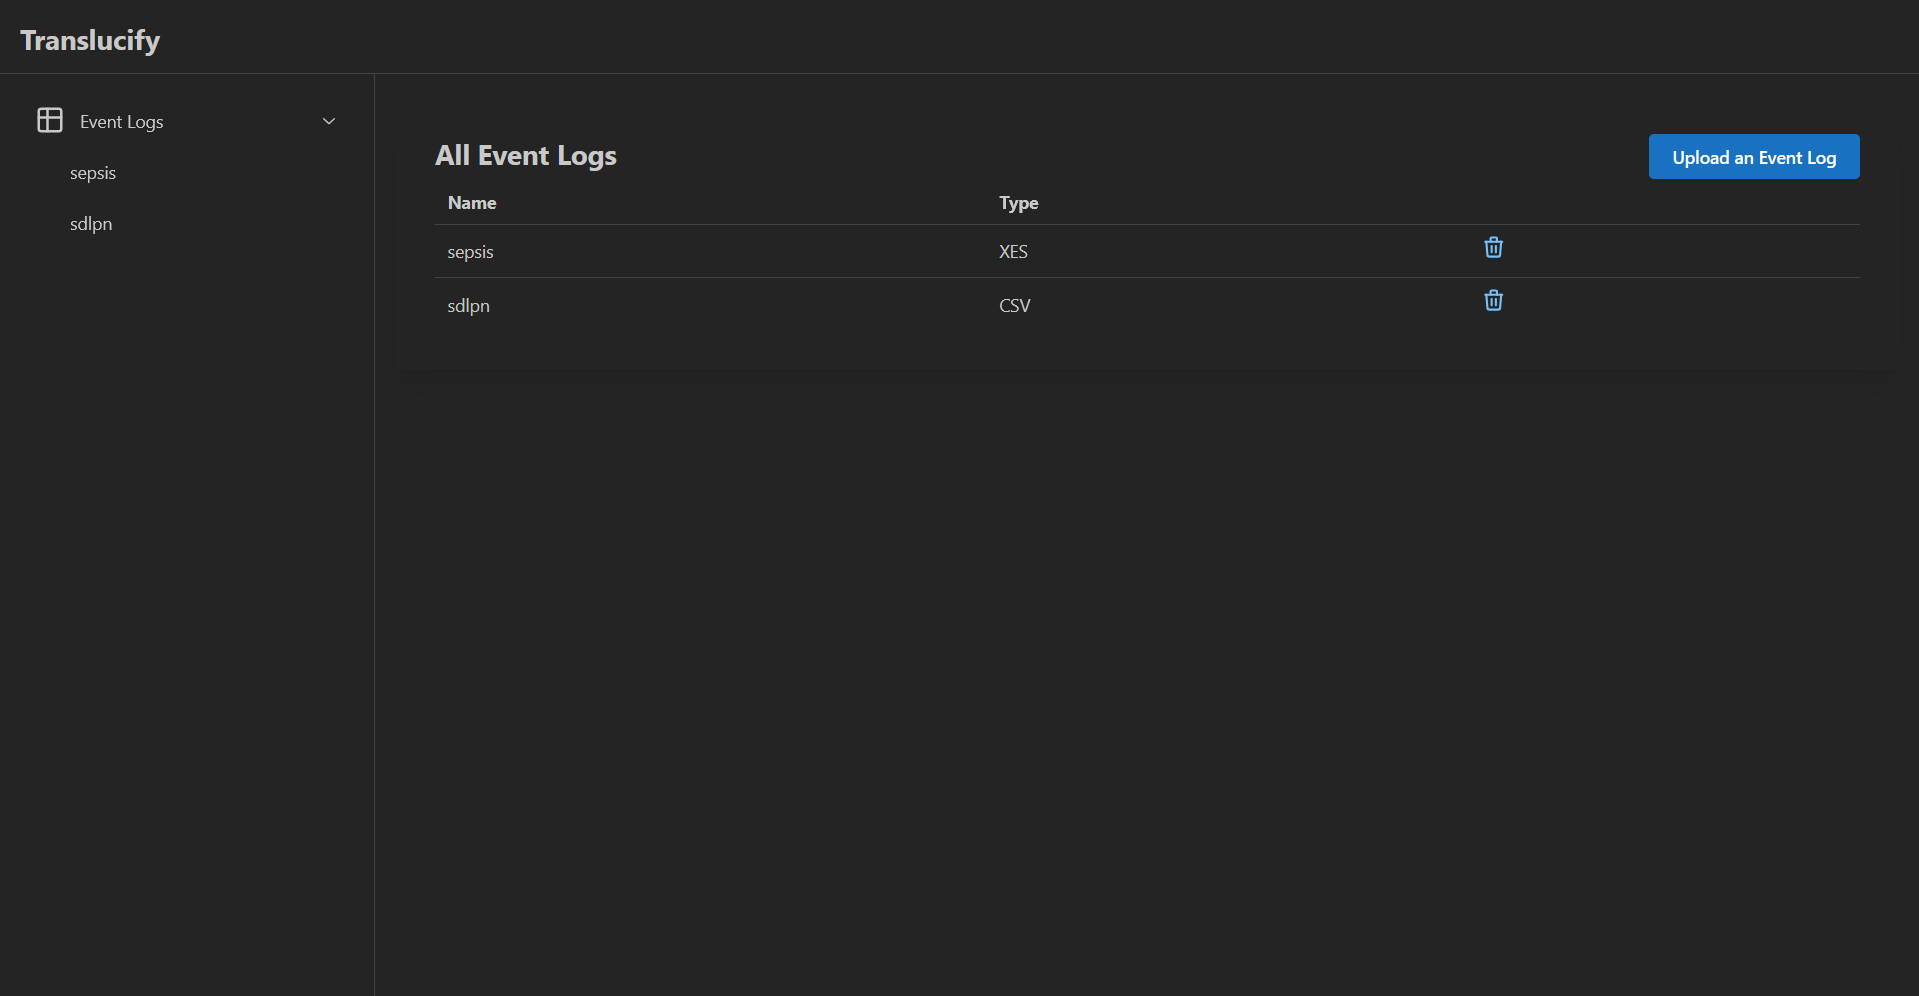
\includegraphics[width=\textwidth]{figures/screenshots/home.png}
    \caption{Home page of \emph{Translucify}.}
    \label{fig:home-page}
\end{figure}

Pressing the $\colorbox{NavyBlue}{\textcolor{white}{\texttt{Upload an Event Log}}}$ button opens a modal used for the event log upload.

The modal wizard consists of two steps. In the first step, the user is prompted to upload the event log data, which can either be in a CSV or an XES format. A name is also a required field for the event log. Although \emph{Translucify} assumes the CSV delimiter to be a semicolon, the user can still specify a custom delimiter if necessary.

The wizard moves onto the second step after clicking on the $\colorbox{NavyBlue}{\textcolor{white}{\texttt{Upload}}}$ button. In the background, the frontend sends a request to the backend in order to save the event log in the database, upon which the backend reads the event log data and returns the column list of the event log. Here, the user can manually select the three fundamental columns for the event log: case ID, activity, and timestamp. After pressing the $\colorbox{NavyBlue}{\textcolor{white}{\texttt{Submit}}}$ button, the user will be subsequently prompted to the event log dashboard of the newly uploaded event log. Figure \ref{fig:upload-modal} illustrates the event log upload modal.

\begin{figure}[H]
    \centering
    \begin{subfigure}[b]{0.45\textwidth}
        \centering
        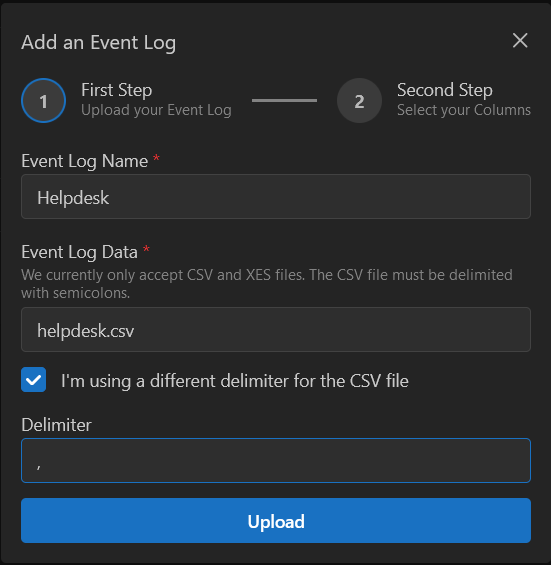
\includegraphics[width=\textwidth]{figures/screenshots/upload1.png}
    \end{subfigure}
    \begin{subfigure}[b]{0.45\textwidth}
        \centering
        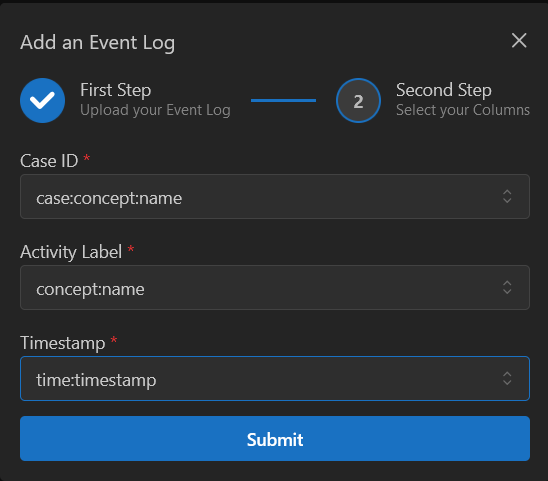
\includegraphics[width=\textwidth]{figures/screenshots/upload2.png}
    \end{subfigure}
    \caption{Event log upload modal consisting of a two-step wizard.}
    \label{fig:upload-modal}
\end{figure}

\subsection{Event Log Dashboard}

\begin{figure}[H]
    \centering
    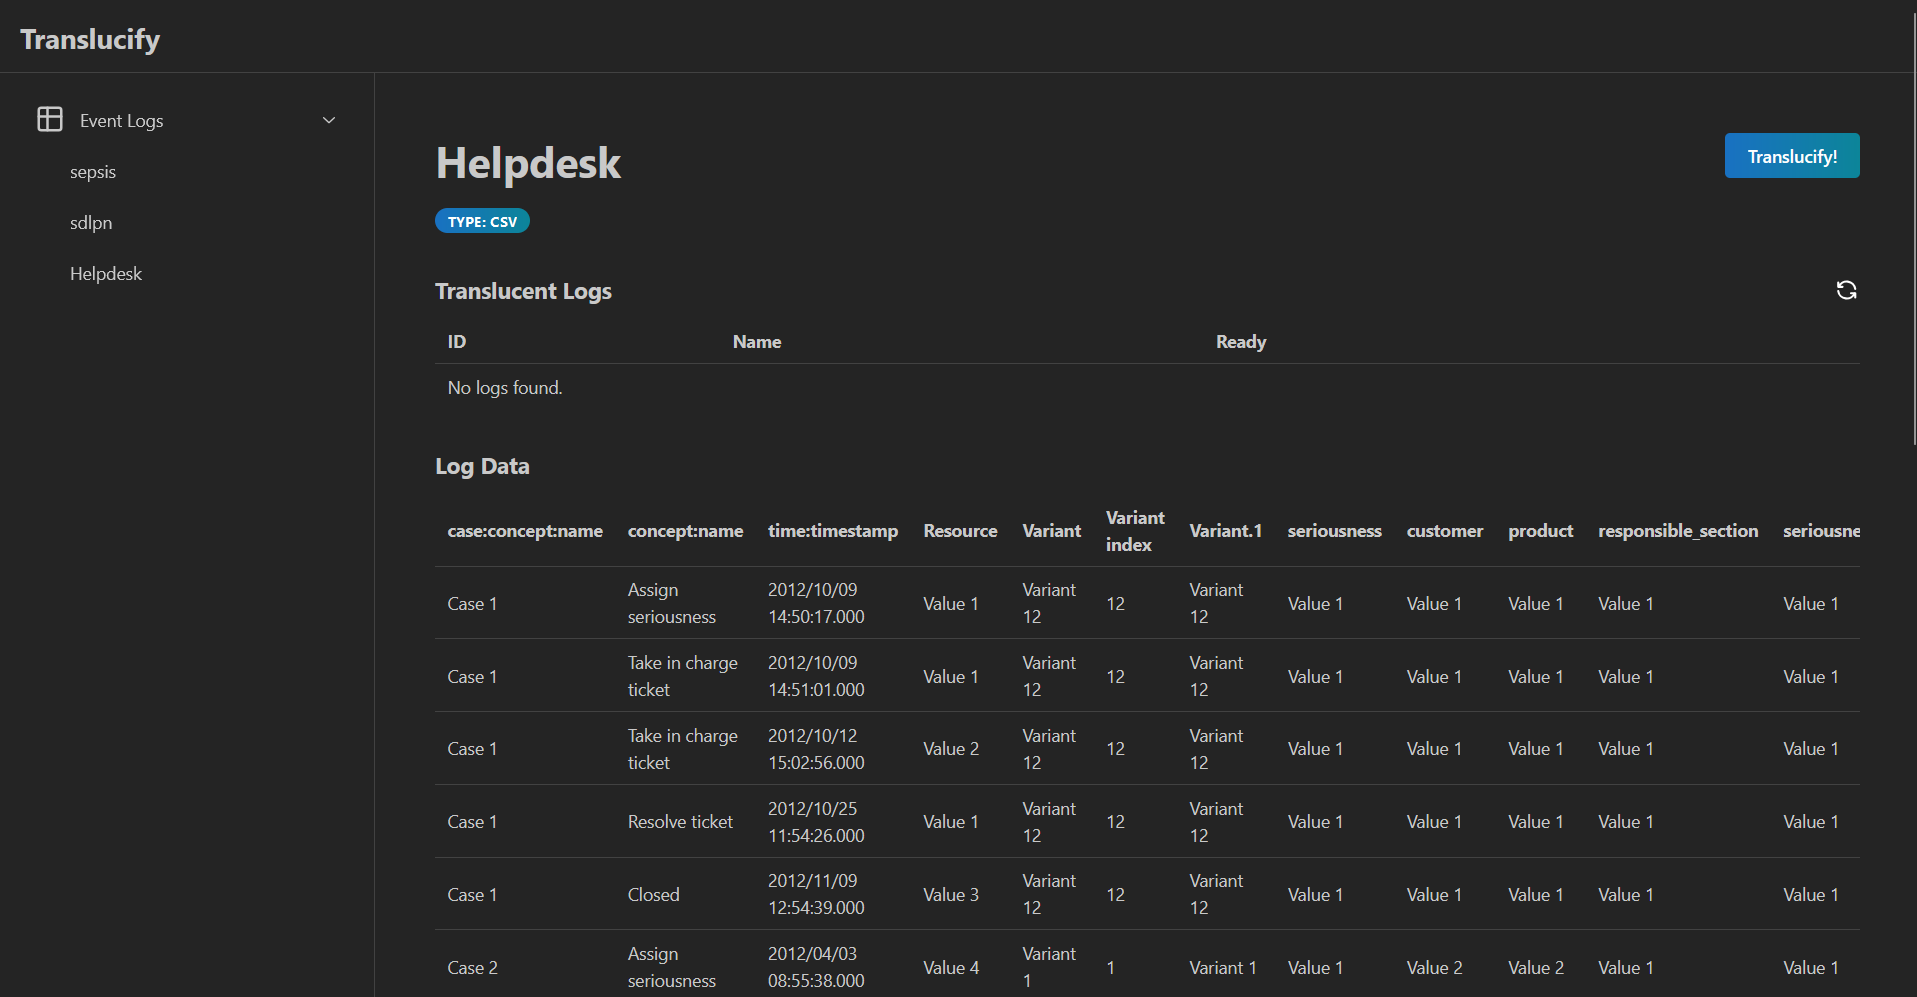
\includegraphics[width=\textwidth]{figures/screenshots/loghome.png}
    \caption{Event log dashboard.}
    \label{fig:log-home}
\end{figure}

\begin{figure}[H]
    \centering
    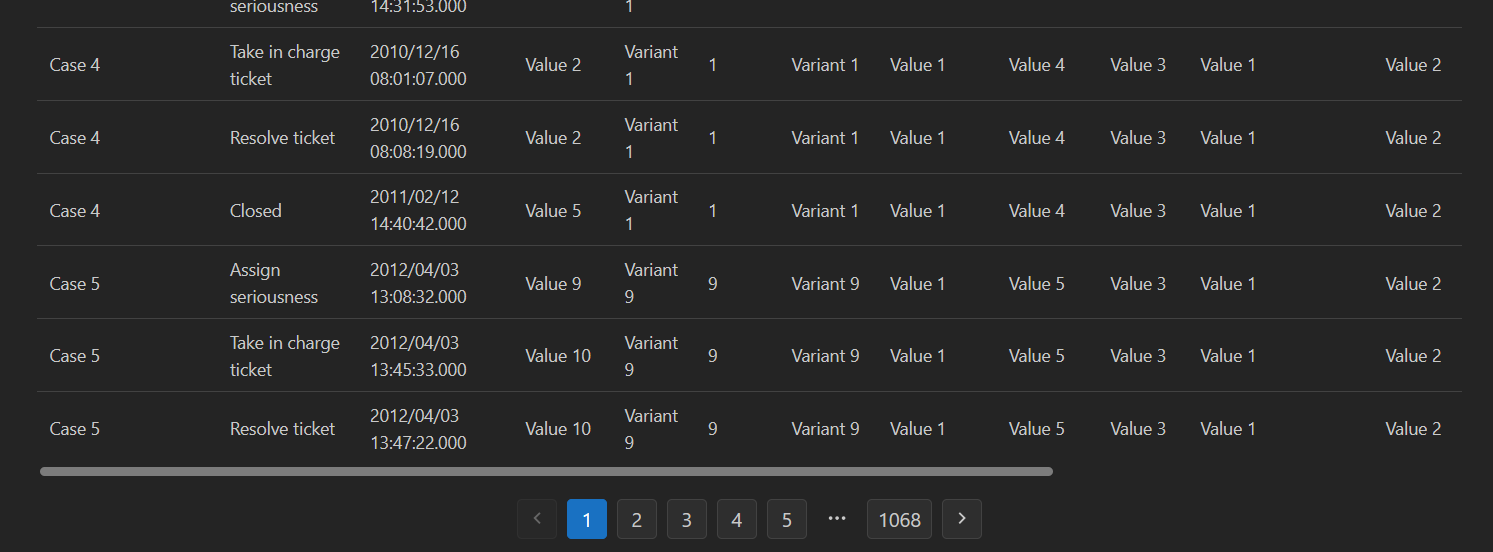
\includegraphics[width=\textwidth]{figures/screenshots/pagination.png}
    \caption{Horizontal scroll and pagination feature for the raw log data.}
    \label{fig:pagination}
\end{figure}

\begin{wrapfigure}{r}{0.4\textwidth}    
    \centering
    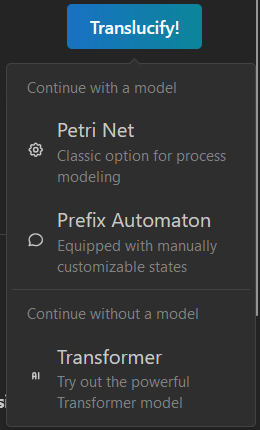
\includegraphics[width=0.35\textwidth]{figures/screenshots/translucify.png}
    \caption{Choice popup.}
    \label{fig:choice-popup}
\end{wrapfigure}

The event log dashboard provides the comprehensive information regarding the specific event log instance and consists of two main sections.

The first section is the translucent log table, in which every generated and to-be-generated translucent event log is registered, listing information such as the generation method and completion status. The download feature enabled the user to download the translucent event log data directly from the table.

The second section is the event log table, which displays the raw event log data in form of a table. During development, we observed frequent browser crashes due to the extensive data size in the table when testing with large event logs. In order to mitigate this, a pagination feature was added to the table. Moreover, the table is horizontally scrollable for event logs with a large column count. Figures \ref{fig:log-home} and \ref{fig:pagination} demonstrate the event log dashboard and the pagination feature, respectively.

Upon clicking the $\colorbox{NavyBlue}{\textcolor{white}{\texttt{Translucify!}}}$ button, the user needs to select between three log generation options: Petri net, prefix automaton, and transformer. Pressing each button navigates the user to the corresponding configuration page. The popup is depicted in Figure \ref{fig:choice-popup}.

\subsection{Configuration Pages}

Petri net and prefix automaton configuration pages share an identical component. The user is first prompted to choose a classifier model between random forests and multivariable regression. Next, the user can select the feature columns to be used for data analysis and subsequently indicate whether the columns are numerical or categorical. Lastly, the user can select the probability threshold for the enabled activities.

\begin{figure}[H]
    \centering
    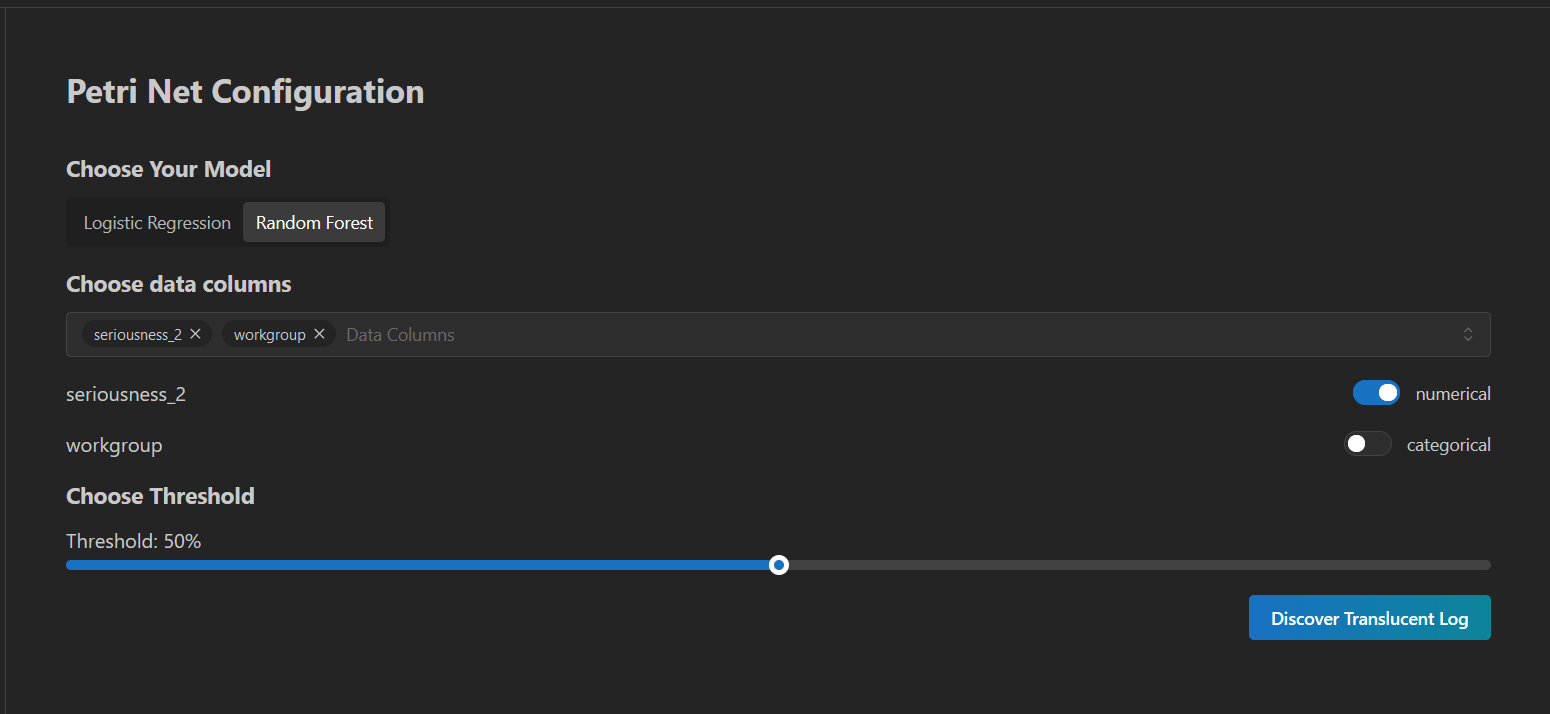
\includegraphics[width=\textwidth]{figures/screenshots/petrinetconfig.png}
    \caption{Petri net configuration page. The random forest model is selected, along with a numerical data column $\texttt{seriousness\_2}$ and a categorical data column $\texttt{workgroup}$. The probability threshold is set to $0.5$.}
    \label{fig:petri-net-config}
\end{figure}

A unique component for the prefix automaton configuration page is the graphical prefix automaton interface, allowing the user to merge states. Figure \ref{fig:pa-merge} illustrates this feature: Upon clicking the checkboxes of the desired states (in this case $\{ \langle a, b, c \rangle \}$ and $\{ \langle a, c, b \rangle \}$) and pressing the $\colorbox{NavyBlue}{\textcolor{white}{\texttt{Merge States}}}$ button, it is visible that the states are now merged into a single state with the description $\{ \langle a, b, c \rangle, \langle a, c, b \rangle \}$. The user can repeat this process until satisfied with his custom finetuning.

\begin{figure}[H]
    \centering
    \begin{subfigure}[b]{\textwidth}
        \centering
        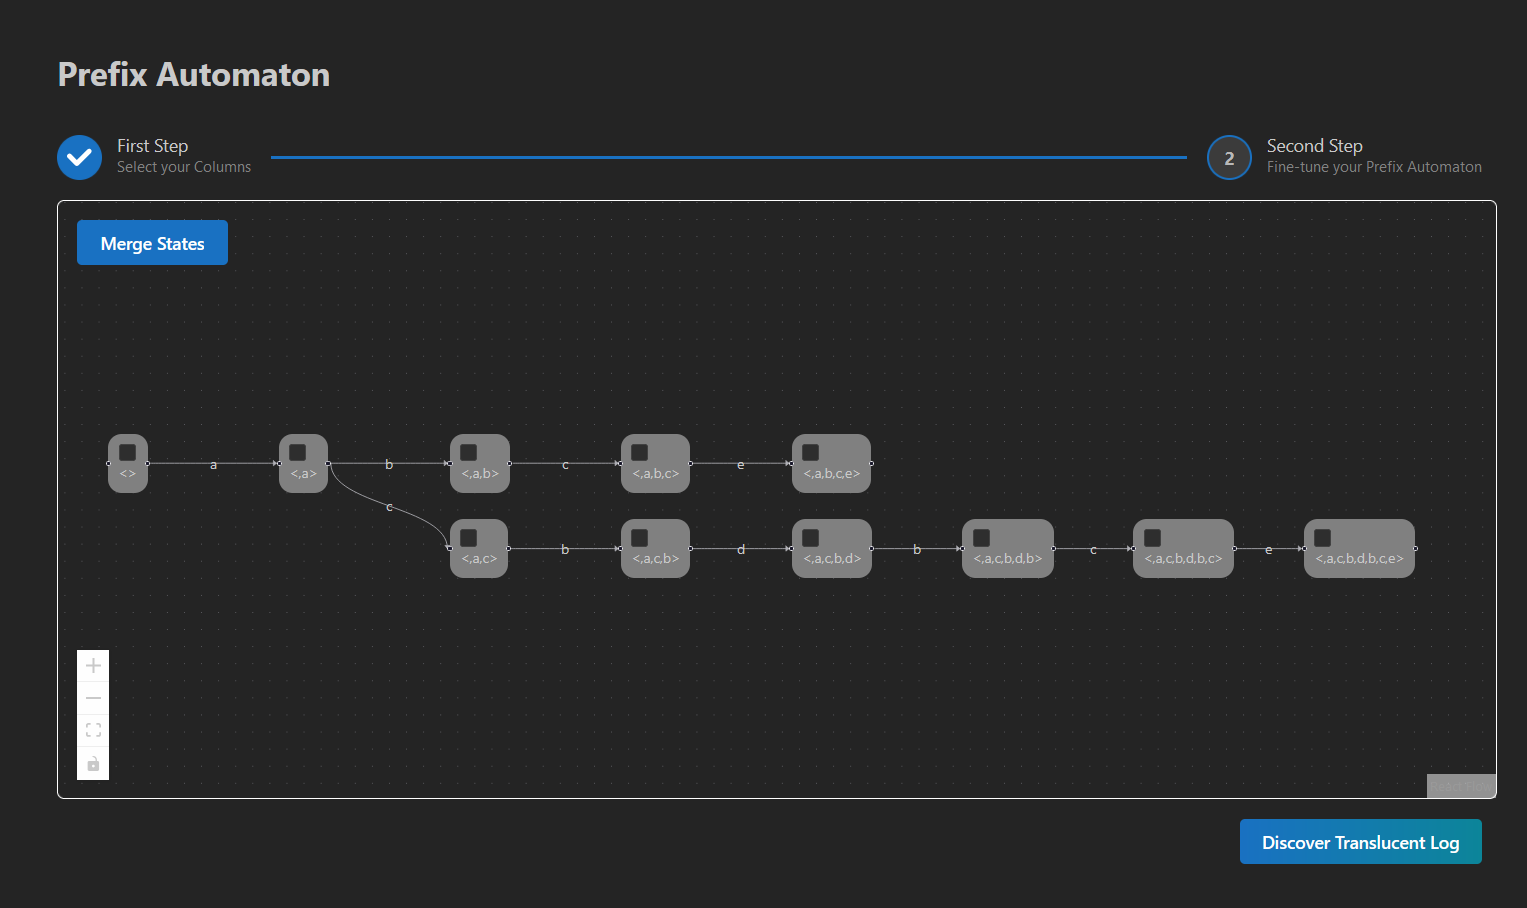
\includegraphics[width=0.8\textwidth]{figures/screenshots/paconfig.png}
    \end{subfigure}
    \begin{subfigure}[b]{\textwidth}
        \centering
        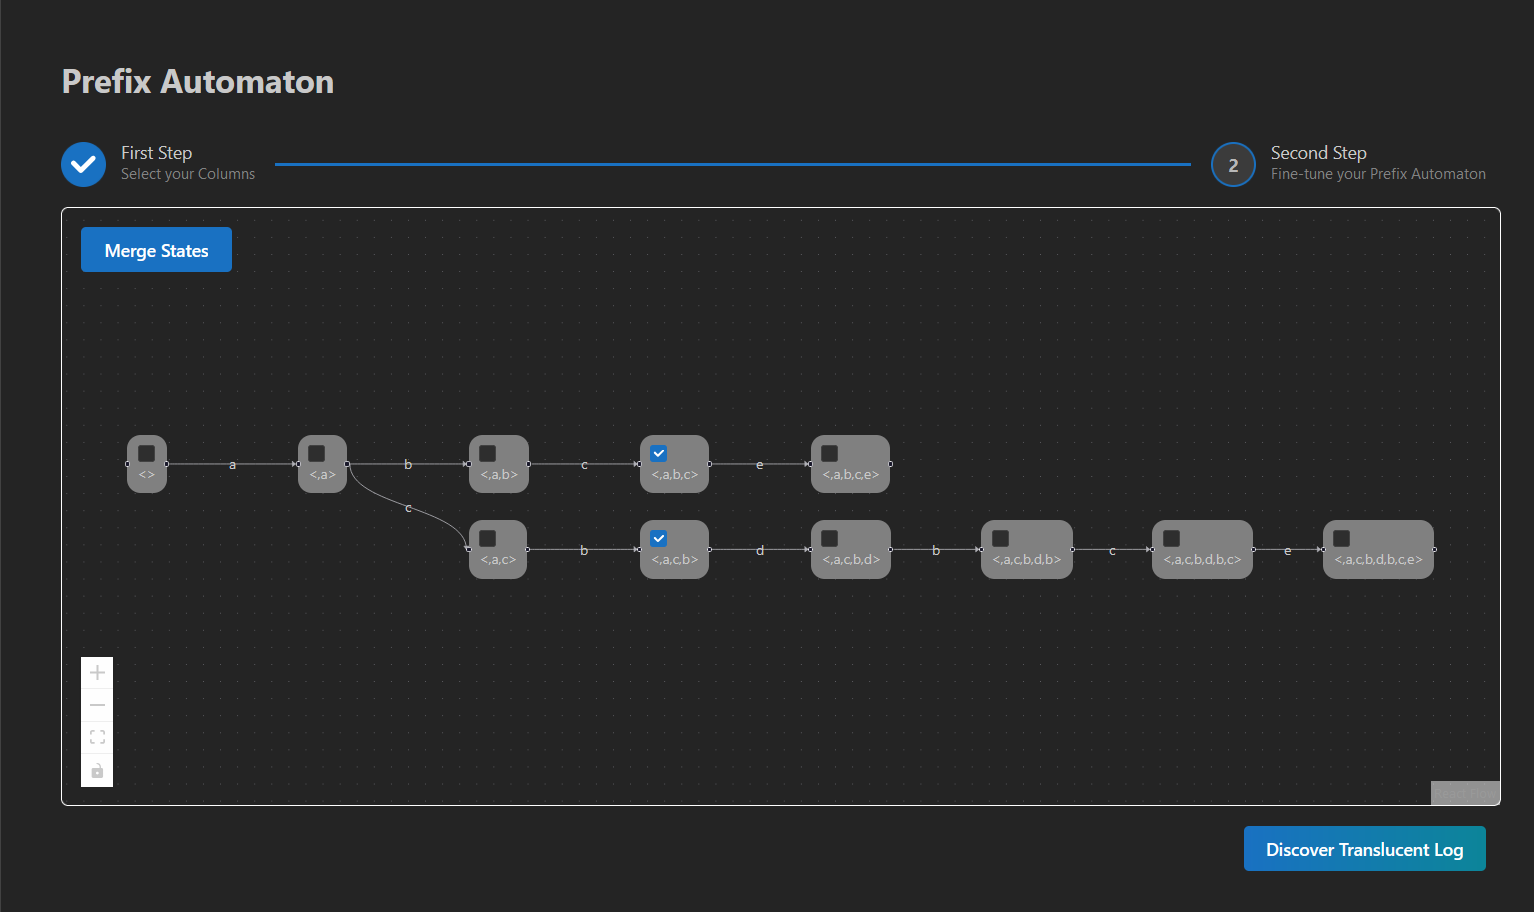
\includegraphics[width=0.8\textwidth]{figures/screenshots/paconfigmerging.png}
    \end{subfigure}
    \begin{subfigure}[b]{\textwidth}
        \centering
        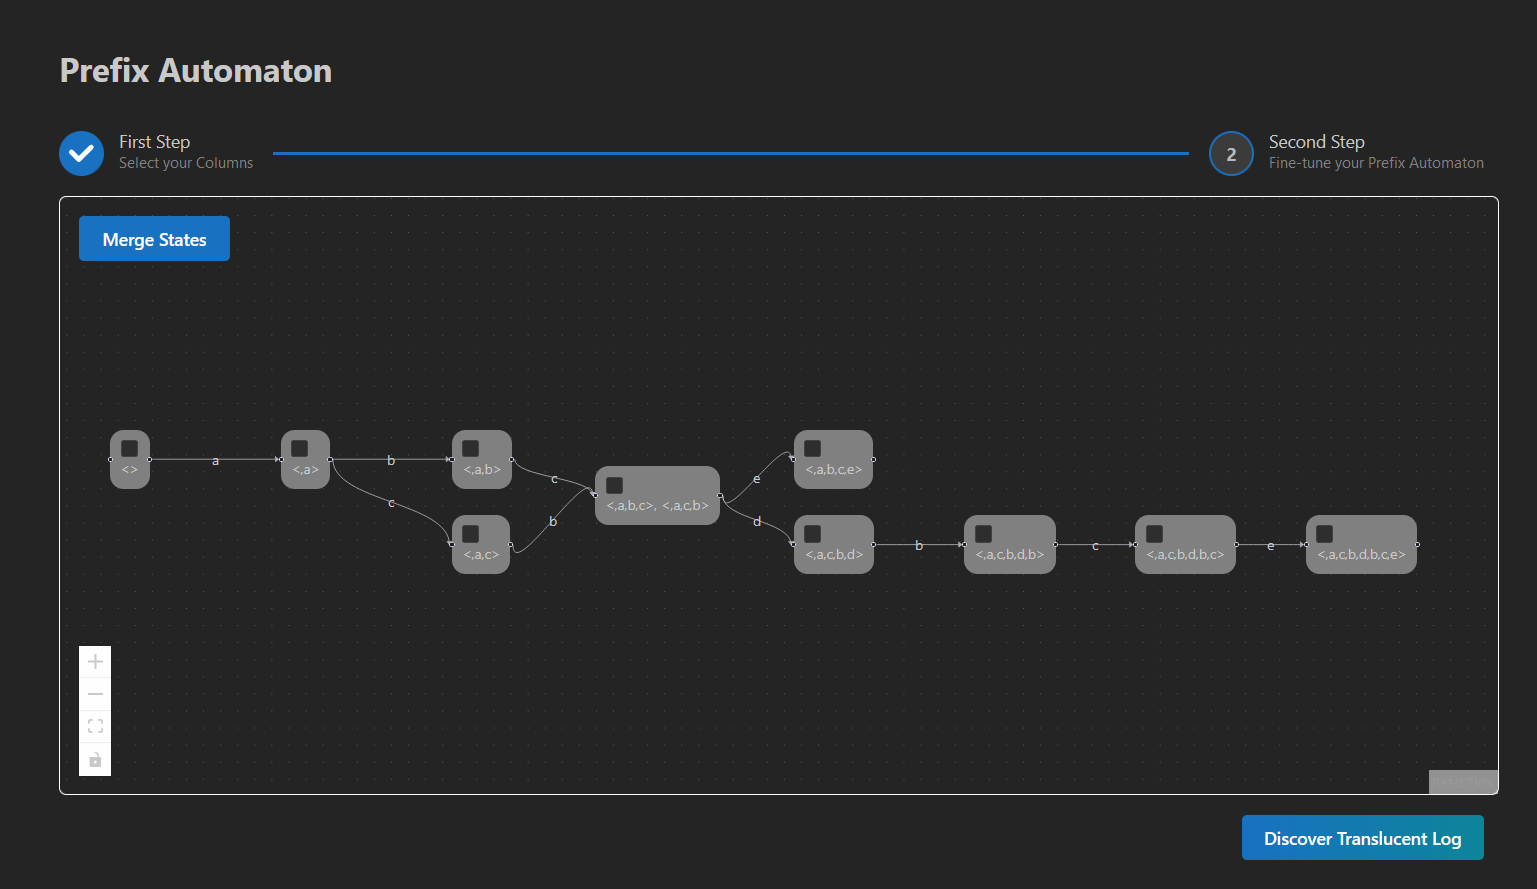
\includegraphics[width=0.8\textwidth]{figures/screenshots/paconfigmerged.png}
    \end{subfigure}
    \caption{Prefix automaton configuration page. The illustrations demonstrate how the state merging feature is used in the frontend.}
    \label{fig:pa-merge}
\end{figure}

The configuration page for transformers is relatively simple as the user only needs to specify the probability threshold.

After the configuration is finished, the user presses the $\colorbox{NavyBlue}{\textcolor{white}{\texttt{Discover Translucent Log}}}$ button. The frontend requests the backend to begin the computation and simultaneously navigates the user back to the event log dashboard. The user waits for the computation to be completed, whose status can be monitored in the translucent log table. With the refresh button, the user can update the completion status. After the computation is finished, the download button will be enabled, allowing the user to download the translucent event log data. Figure \ref{fig:translucent-log-status} shows how the status indicators are displayed in the translucent log table.

\begin{figure}[H]
    \centering
    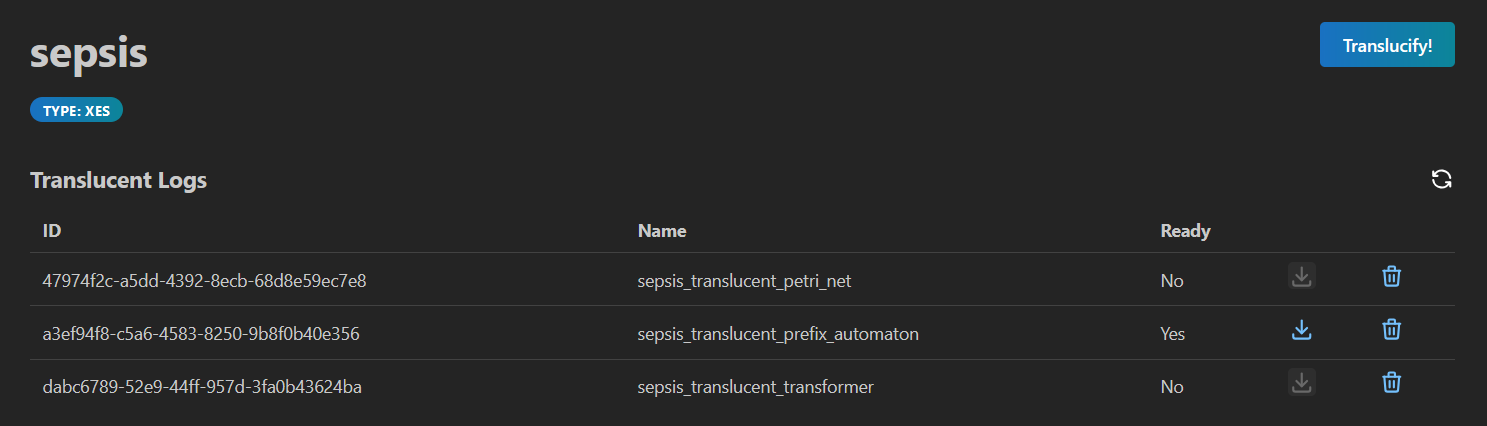
\includegraphics[width=\textwidth]{figures/screenshots/status.png}
    \caption{Status indicators in the translucent log table. The lit blue download button is visible for completed computations.}
    \label{fig:translucent-log-status}
\end{figure}

